%%%%%%%%%%%%%%%%%%%%%%%%%%%%%%%%%%%%%%%%%%%%%%%%%%%%%%%%%%%%%%%%%%%%%%%%%%%%%%%%%%%%%
%																					%
%	TRABAJO: Proyecto Integrador													%
%																					%
%		Titulo: 	Desarrollo de IP cores con procesamiento de Redes de Petri 		%
%					Temporales para sistemas multicore en FPGA						%
%																					%
%		Autores:	Juli�n Nonino													%
%					Carlos Renzo Pisetta											%
%		Director:	Orlando Micolini												%
%																					%
%	Parte: Apendices																%
%	Capitulo: Creacion de un nuevo IP core											%
%	Archivo: creacion_IP_core.tex													%
%																					%
%%%%%%%%%%%%%%%%%%%%%%%%%%%%%%%%%%%%%%%%%%%%%%%%%%%%%%%%%%%%%%%%%%%%%%%%%%%%%%%%%%%%%

% Path Imagenes: ./apendices/creacion_IP_core/img
% Nombre predeterminado imagenes: ipcorexx
%	xx es el numero de imagen

\chapter{Creaci�n de un nuevo IP core}
	\label{ap:creacion_IP_core}

	La herramienta \emph{Xilinx Platform Studio (XPS)} \cite{xilinx_edk} provee un asistente 
	para la creaci�n de un nuevo IP core. A continuaci�n, se mostrar� paso a paso el uso del
	mismo.
	\begin{figure}[H]
		\centering
		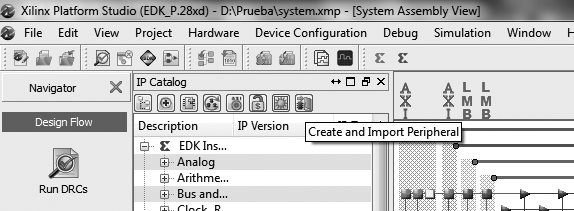
\includegraphics[width=0.5\linewidth,keepaspectratio]{./apendices/creacion_IP_core/img/ipcore01}
		\caption{Inicio del asistente de creaci�n de IP cores}
		\label{fig:ipcore01}
	\end{figure}
	En la Figura \ref{fig:ipcore01}, se observa como se puede acceder al asistente de creaci�n 
	de IP cores. En la siguiente (Figura \ref{fig:ipcore02}), se muestra la ventana principal 
	del asistente.
	\begin{figure}[H]
		\centering
		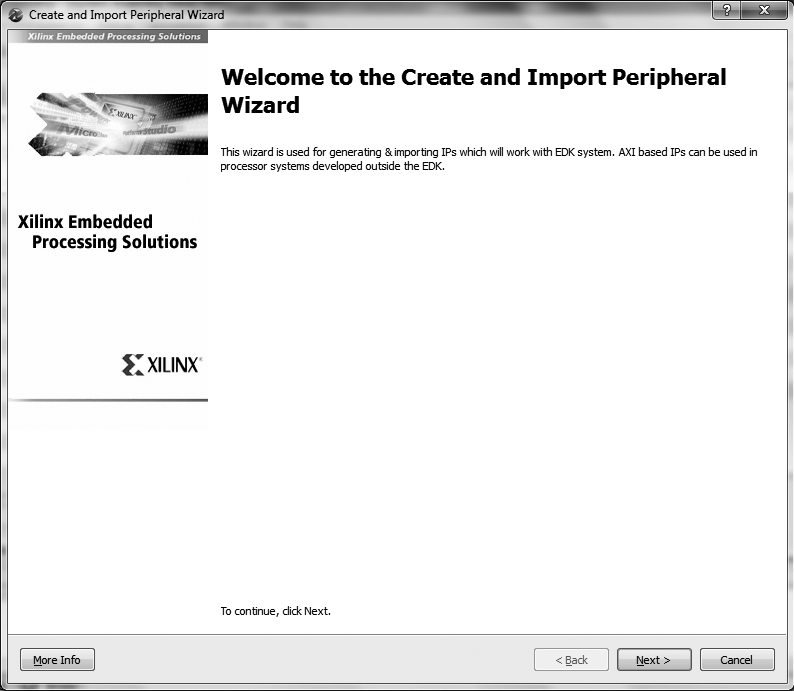
\includegraphics[width=0.4\linewidth,keepaspectratio]{./apendices/creacion_IP_core/img/ipcore02}
		\caption{Ventana principal del asistente de creaci�n de IP cores}
		\label{fig:ipcore02}
	\end{figure}
	Haciendo click en \emph{Next} se avanzara en las etapas del asistente y se ir� conFigurando distintos 
	aspectos de nuevo IP core.
	\newpage
	
	En la siguiente ventana (Figura \ref{fig:ipcore03}) se debe elegir si se crear� un nuevo IP core o se 
	importar� uno ya existente.
	
	\begin{figure}[H]
		\centering
		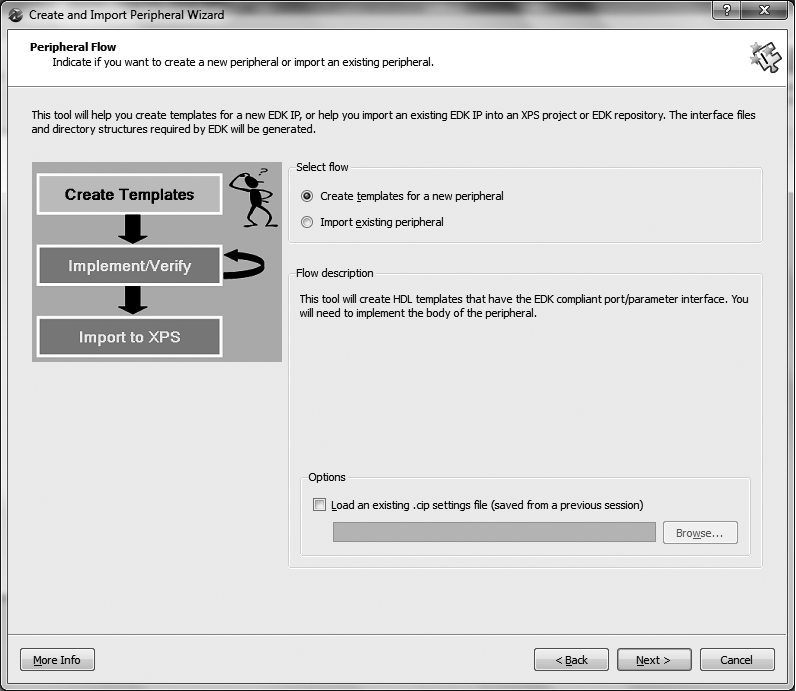
\includegraphics[width=0.7\linewidth,keepaspectratio]{./apendices/creacion_IP_core/img/ipcore03}
		%\caption{}
		\label{fig:ipcore03}
	\end{figure}
	
	Luego, se debe determinar si el nuevo IP core se guardar� dentro del proyecto o en alg�n repositorio 
	del usuario (Figura \ref{fig:ipcore04}).
	
	\begin{figure}[H]
		\centering
		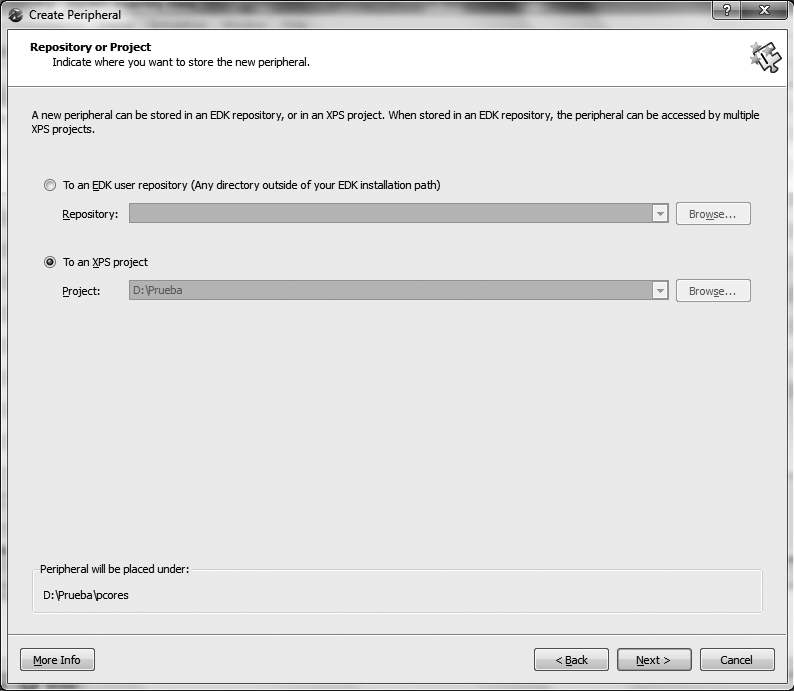
\includegraphics[width=0.7\linewidth,keepaspectratio]{./apendices/creacion_IP_core/img/ipcore04}
		%\caption{}
		\label{fig:ipcore04}
	\end{figure}
	\newpage
	El paso siguiente es darle un nombre al nuevo IP core, determinar la versi�n del mismo y brindar una 
	descripci�n (Figura \ref{fig:ipcore05}).
	
	\begin{figure}[H]
		\centering
		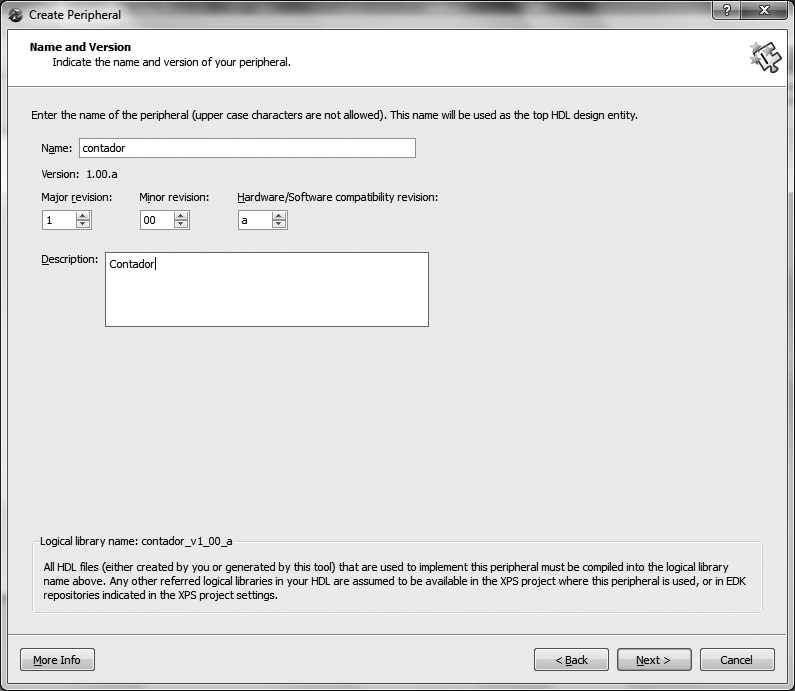
\includegraphics[width=0.7\linewidth,keepaspectratio]{./apendices/creacion_IP_core/img/ipcore05}
		%\caption{}
		\label{fig:ipcore05}
	\end{figure}
	
	Luego, hay elegir el bus a trav�s del cual el nuevo IP core se conectara al sistema (figra \ref{fig:ipcore06}).
	
	\begin{figure}[H]
		\centering
		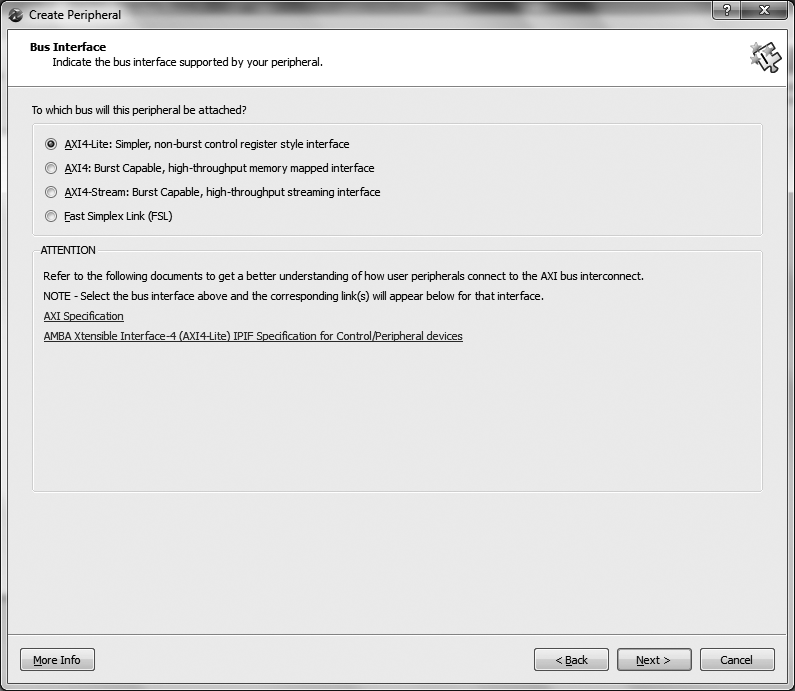
\includegraphics[width=0.7\linewidth,keepaspectratio]{./apendices/creacion_IP_core/img/ipcore06}
		%\caption{}
		\label{fig:ipcore06}
	\end{figure}	
	\newpage
	Posteriormente, se deben conFigurar las interfaces del nevo IP core Figura \ref{fig:ipcore07}.
	En esta etapa se eligen par�metros relacionados con la configuraci�n de la interfaz entre el bus 
	y el IP core. Entre estas opciones se encuentran, soporte para que el IP core se comporte como 
	\emph{master} en el bus. Incluir registros accesibles por software, un reset accesible por software, 
	etc�tera.
	\begin{figure}[H]
		\centering
		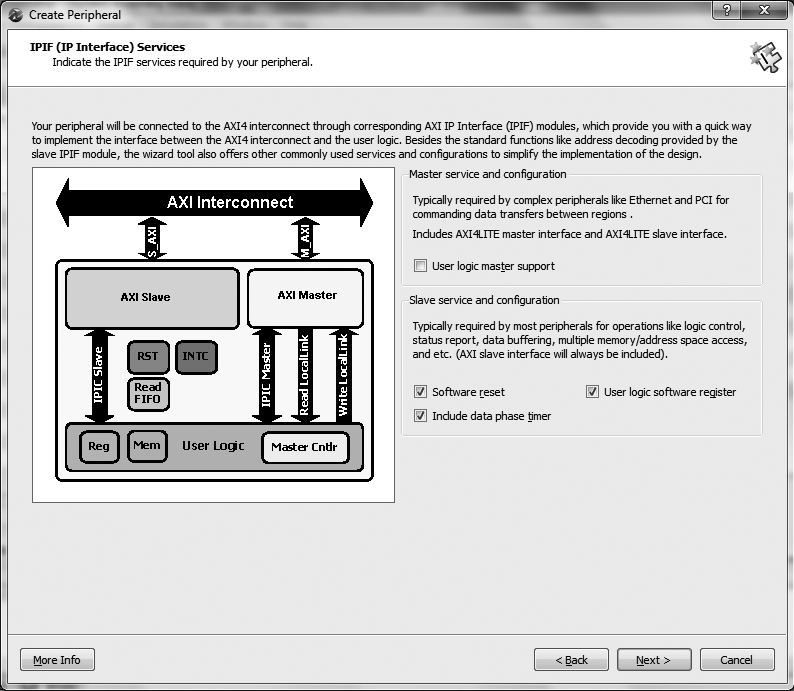
\includegraphics[width=0.65\linewidth,keepaspectratio]{./apendices/creacion_IP_core/img/ipcore07}
		%\caption{}
		\label{fig:ipcore07}
	\end{figure}		
	Despu�s, es posible elegir la cantidad de registros accesibles del IP core (Figura \ref{fig:ipcore08}).
	\begin{figure}[H]
		\centering
		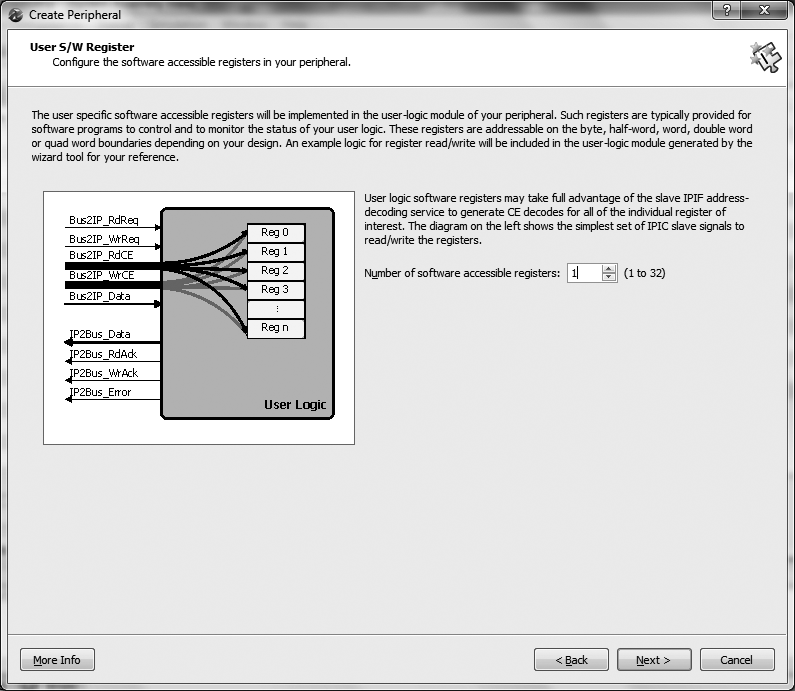
\includegraphics[width=0.65\linewidth,keepaspectratio]{./apendices/creacion_IP_core/img/ipcore08}
		%\caption{}
		\label{fig:ipcore08}
	\end{figure}	
	\newpage
	El siguiente paso es elegir que puertos desde o hacia el bus se desean que sean accesibles desde el 
	IP core (Figura \ref{fig:ipcore09}).
	\begin{figure}[H]
		\centering
		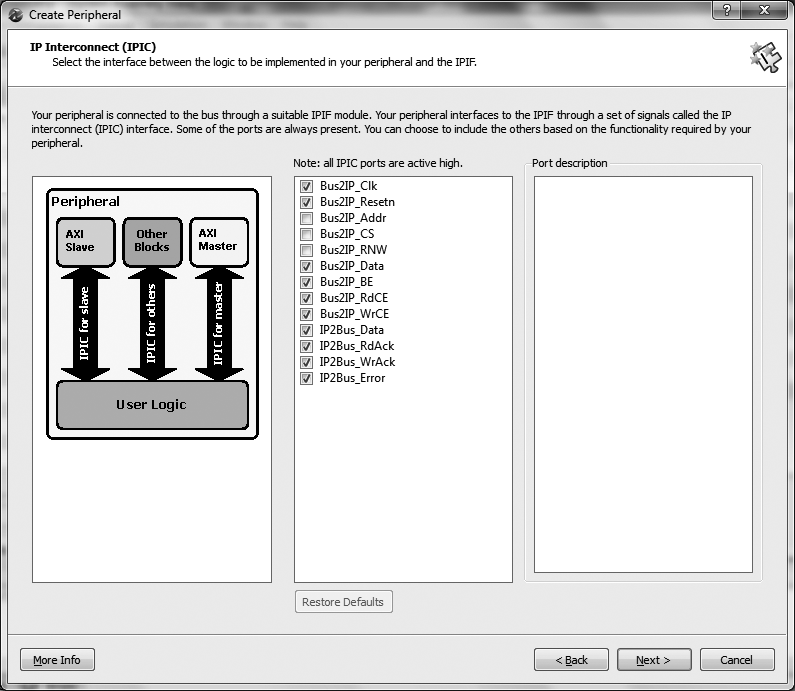
\includegraphics[width=0.7\linewidth,keepaspectratio]{./apendices/creacion_IP_core/img/ipcore09}
		%\caption{}
		\label{fig:ipcore09}
	\end{figure}
	Luego, se debe determinar si se desea incluir un template para simular el IP core generado 
	(Figura \ref{fig:ipcore10}).
	\begin{figure}[H]
		\centering
		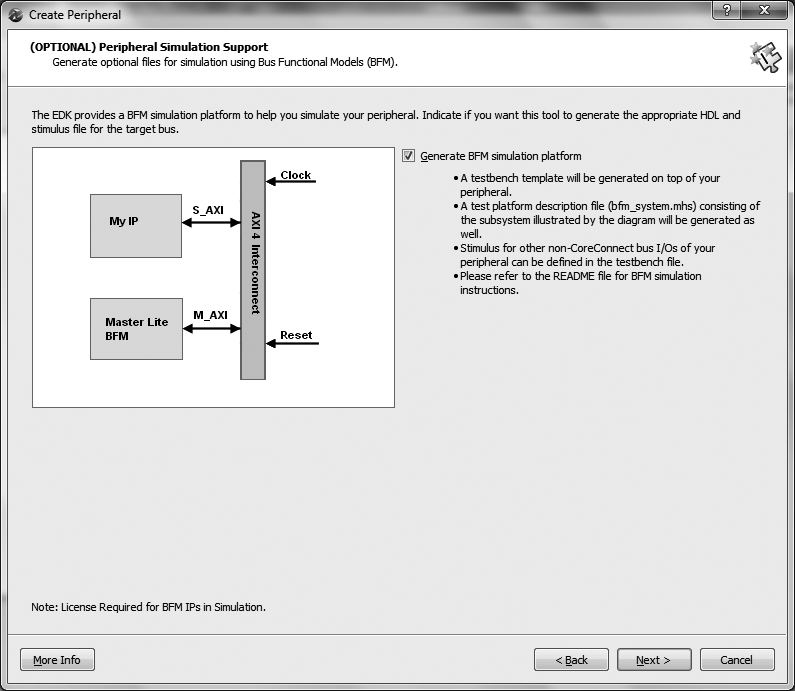
\includegraphics[width=0.7\linewidth,keepaspectratio]{./apendices/creacion_IP_core/img/ipcore10}
		%\caption{}
		\label{fig:ipcore10}
	\end{figure}
	\newpage
	Posteriormente, se seleccionan opciones relacionadas con la implementaci�n de la l�gica del IP core
	(Figura \ref{fig:ipcore11}). Por ejemplo, se puede decidir si el archivo \emph{user logic} se 
	implementar� en Verilog o en VHDL, si se desea crear un proyecto ISE para poder editar el IP core 
	desde esta herramienta y/o generar templates con los drivers para facilitar la implementaci�n del software. 
	\begin{figure}[H]
		\centering
		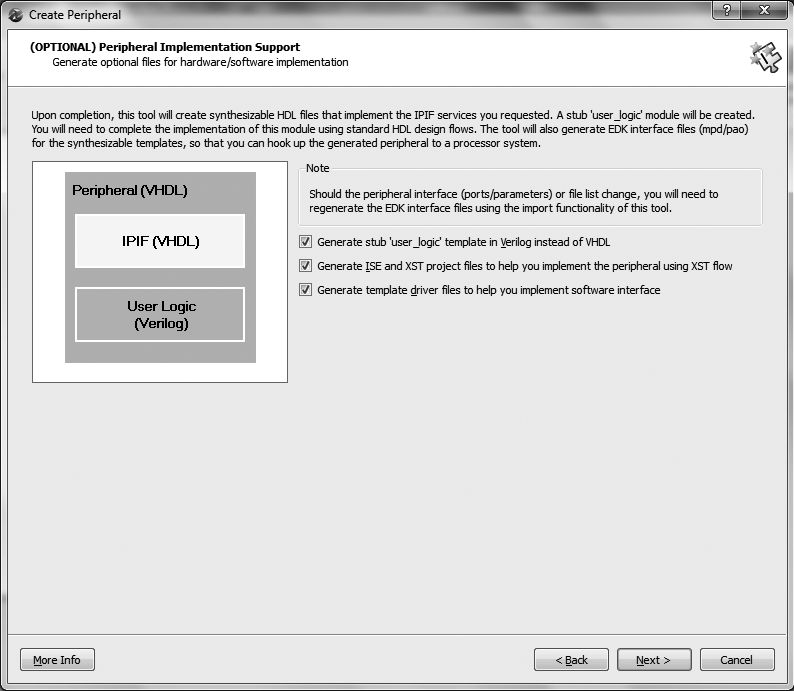
\includegraphics[width=0.65\linewidth,keepaspectratio]{./apendices/creacion_IP_core/img/ipcore11}
		%\caption{}
		\label{fig:ipcore11}
	\end{figure}	
	En la p�gina final (Figura \ref{fig:ipcore12}), Se muestra un resumen de las opciones elegidas.
	\begin{figure}[H]
		\centering
		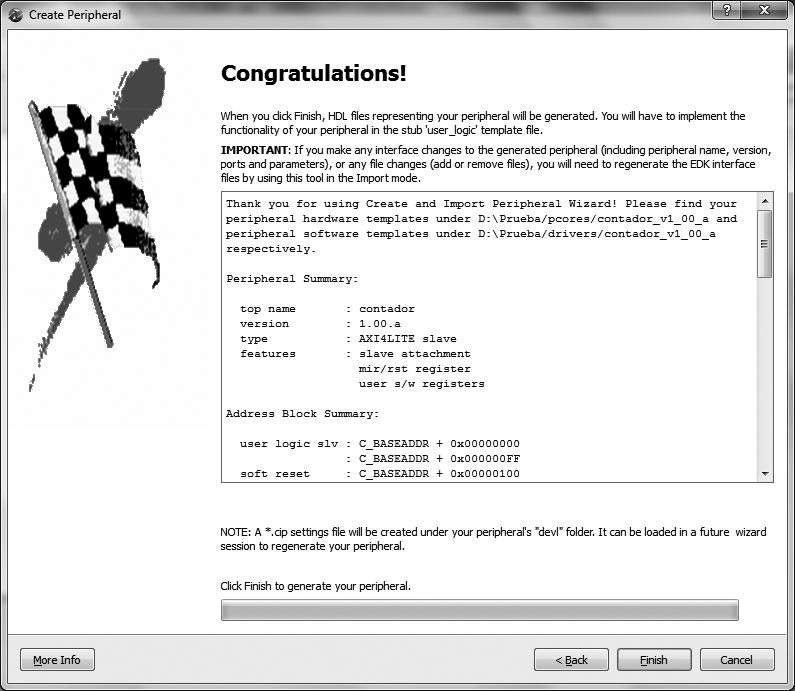
\includegraphics[width=0.65\linewidth,keepaspectratio]{./apendices/creacion_IP_core/img/ipcore12}
		%\caption{}
		\label{fig:ipcore12}
	\end{figure}
	\newpage
	Haciendo click en \emph{Finish} el IP core queda agregado al repositorio (Figura \ref{fig:ipcore13}).
	\begin{figure}[H]
		\centering
		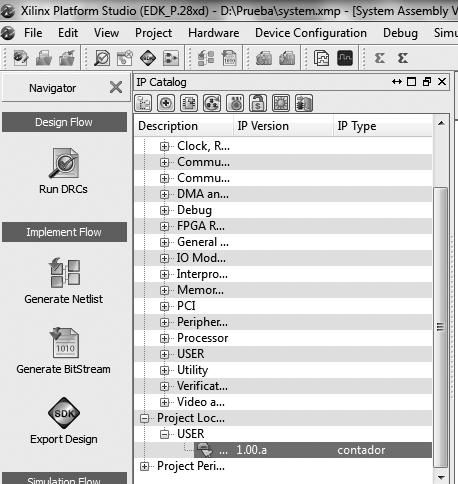
\includegraphics[width=0.75\linewidth,keepaspectratio]{./apendices/creacion_IP_core/img/ipcore13}
		%\caption{}
		\label{fig:ipcore13}
	\end{figure}
	Luego, haciendo click derecho en el IP core, se puede seleccionar la opci�n para agregarlo al sistema. 
	Al hacer esto se muestra la siguiente ventana (Figura \ref{fig:ipcore14}).
	\begin{figure}[H]
		\centering
		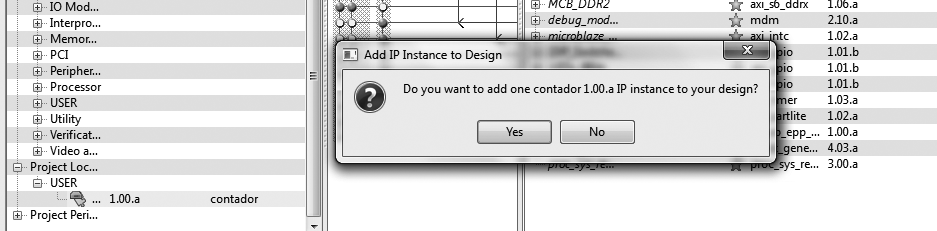
\includegraphics[width=1\linewidth,keepaspectratio]{./apendices/creacion_IP_core/img/ipcore14}
		%\caption{}
		\label{fig:ipcore14}
	\end{figure}
	\newpage
	Luego de seleccionar que desea agregarse el IP core al sistema, se muestra una ventana para realizar 
	conFiguraciones en los par�metros del IP core antes de agregarlo al sistema (Figura \ref{fig:ipcore15}). 
	\begin{figure}[H]
		\centering
		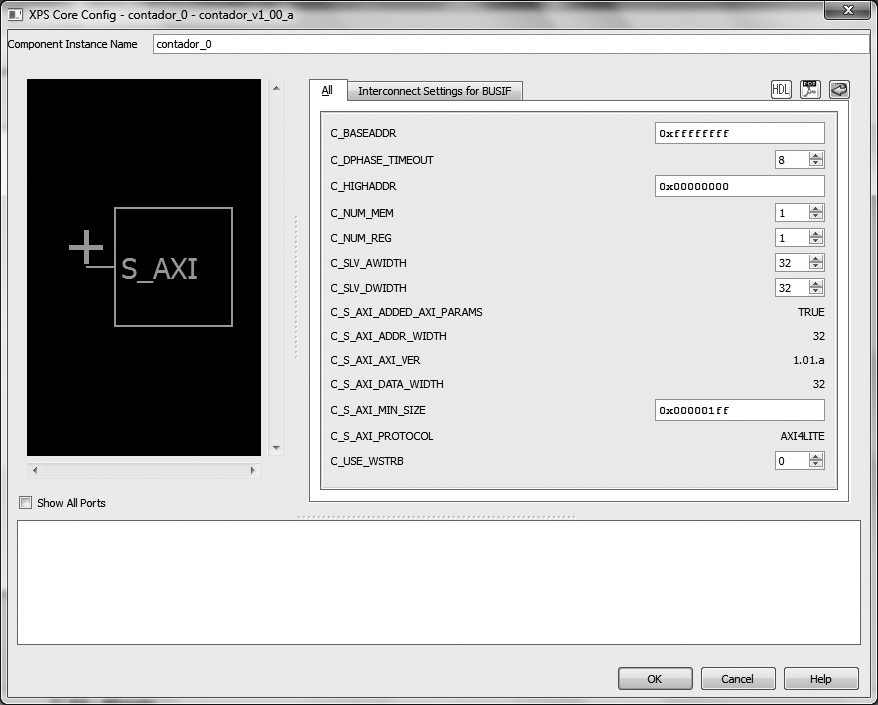
\includegraphics[width=0.8\linewidth,keepaspectratio]{./apendices/creacion_IP_core/img/ipcore15}
		%\caption{}
		\label{fig:ipcore15}
	\end{figure}
	Terminado de conFigurar el IP core se muestra la siguiente ventana (Figura \ref{fig:ipcore16}) que 
	pregunta si se desea conectar el IP core al procesador del sistema o si el usuario realizar� manualmente 
	todas las conexiones.
	\begin{figure}[H]
		\centering
		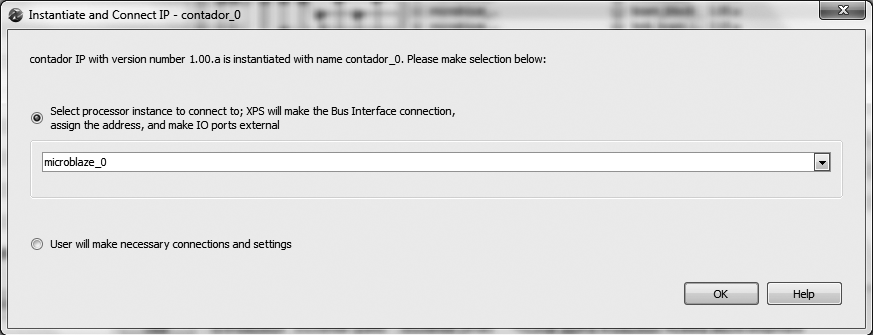
\includegraphics[width=1\linewidth,keepaspectratio]{./apendices/creacion_IP_core/img/ipcore16}
		%\caption{}
		\label{fig:ipcore16}
	\end{figure}
	\newpage
	Finalmente, \textbf{\emph{el IP core ya se encuentra agregado al sistema}}(Figura \ref{fig:ipcore17}).
	\begin{figure}[H]
		\centering
		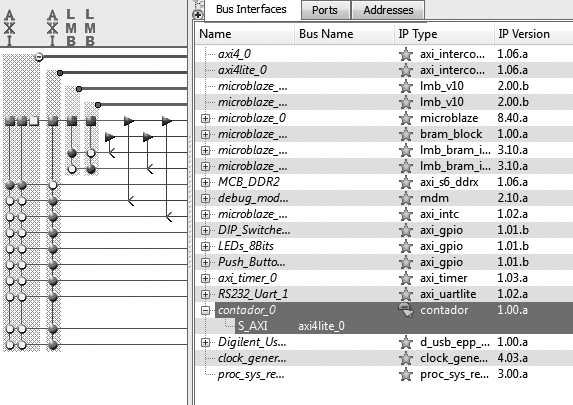
\includegraphics[width=1\linewidth,keepaspectratio]{./apendices/creacion_IP_core/img/ipcore17}
		%\caption{}
		\label{fig:ipcore17}
	\end{figure}